\documentclass[c]{beamer}
\usepackage{org-preamble}
\usepackage[cpp_teaching]{slide-style}
\usepackage{minted}
\newcommand{\inline}[1]{\mintinline[breaklines]{c++}{#1}}      
\newcommand{\ttb}[1]{\textcolor{black}{#1}}
\newcommand{\ttg}[1]{\textcolor{green}{#1}}                
\usetheme{default}

\title{Héritage}


\begin{document}

\maketitle
\def\theFancyVerbLine{%
  \color{white}\sffamily\tiny\arabic{FancyVerbLine}%
        {\tikz[remember picture,overlay]\node(minted-\arabic{FancyVerbLine}){};}%
}
\tikzset{codeblock/.style={color=#1!50,rounded corners=0.5ex, opacity=0.2, fill}}



\begin{frame}[fragile]{Introduction}
\begin{itemize}
\item L'héritage est une relation hiérarchique entre classes. C'est un mécanisme permettant de construire une classe à partir d'une autre classe existante.
\end{itemize}

\begin{center}
  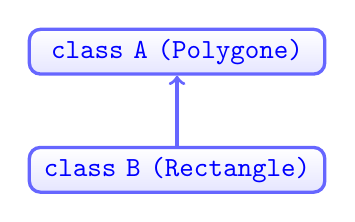
\begin{tikzpicture}[
      grow=down,
      linet/.style={very thick,draw=blue!60,
        shorten >=0pt, shorten <=0pt, <-},
      punkt/.style={rectangle, rounded corners, shade, top color=white,
        bottom color=blue!10, draw=blue!60, very thick,
        text centered, text width=9.5em}
    ]
    \ttfamily\color{blue}
    \path (0,0)    node(a) [punkt] {class A (Polygone)}
          (0,-1.5) node(b) [punkt] {class B (Rectangle)};
    \draw[linet] (a) -- (b);
  \end{tikzpicture}
\end{center}
\end{frame}

%------------------------------------------------------------------------

\begin{frame}[fragile]{Une classe \texttt{B} héritant d'une classe \texttt{A}}
 \begin{center}
  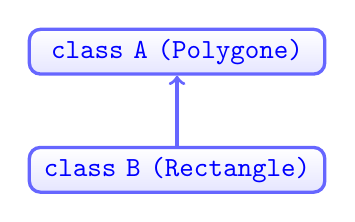
\begin{tikzpicture}[
      grow=down,
      linet/.style={very thick,draw=blue!60,
        shorten >=0pt, shorten <=0pt, <-},
      punkt/.style={rectangle, rounded corners, shade, top color=white,
        bottom color=blue!10, draw=blue!60, very thick,
        text centered, text width=9.5em}
    ]
    \ttfamily\color{blue}
    \path (0,0)    node(a) [punkt] {class A (Polygone)}
    (0,-1.5) node(b) [punkt] {class B (Rectangle)};
    \draw[linet] (a) -- (b);
  \end{tikzpicture}
\end{center}

\begin{itemize}
\item La classe \texttt{B} hérite de tous les membres (attributs et méthodes) de la classe \texttt{A}
\item Les méthodes (et fonctions amies) de \texttt{B} ont accès aux membres publics et protégés de \texttt{A}
\end{itemize}

\pause

\begin{itemize}
\item Ainsi, la classe \texttt{B} est basée sur la classe \texttt{A} mais peut également ajouter
de nouveaux membres ainsi que de nouvelles méthodes propres à sa fonction :

\begin{itemize}
\item la classe \texttt{A} que l'on appellera \structure{classe mère ou de base} est \structure{une
généralisation/abstraction} de \texttt{B},

\item la classe \texttt{B} que l'on dit \structure{dérivée ou classe fille} de \texttt{A} est donc \structure{une
spécialisation} de \texttt{A}.
\end{itemize}
\end{itemize}
\end{frame}


%------------------------------------------------------------------------

\begin{frame}[fragile]{Définition : héritage simple/multiple, composition}
On distingue les deux liens logiques que sont l'héritage et la composition:

\begin{description}
\item[{Composition}] relation de type \structure{\textbf{a un (verbe avoir)}}; la classe \texttt{Polygone} a
un ensemble d'objets de type \texttt{point}, 
\item[{Héritage\footnote{On devrait parler de \textbf{sous-typage}; l'héritage n'étant qu'une façon de faire du sous-typage.}}] relation de type \structure{\textbf{est un (verbe être)}}; un \texttt{Rectangle} est un
\texttt{Polygone}, une \texttt{Voiture} est un \texttt{Véhicule}.
\end{description}

\bigskip

\begin{description}
\item[{Héritage simple}] : une classe n'hérite que d'une seule classe, 
\item[{Héritage multiple}] : une classe hérite de plus d'une classe (plus délicat à mettre en oeuvre) 
\end{description}

\end{frame}

%----------------------------------------------------------------------

\begin{frame}[fragile]{Notions d'héritage simple}
 \begin{minted}[fontsize=\footnotesize,samepage,mathescape,xrightmargin=0.5cm,xleftmargin=0.5cm]{c++}
class Polygone {
public:
  Polygone (const unsigned int nbr_segment); 
protected:
  unsigned int m_nombre_segment;
};

class Rectangle : public Polygone {
public:
  Rectangle (const double longueur, const double largeur);
private:
  double m_longueur;
  double m_largeur;
};
\end{minted}

\pause
\begin{itemize}
\item La relation d'héritage est matérialisée par l'usage de la directive \structure{\texttt{public
  Polygone}}
\end{itemize}
\pause
\begin{itemize}
\item Le mot-clé \structure{\texttt{protected}} autorise la classe dérivée (ici \texttt{Rectangle}) à accéder
aux membres de la classe de base (ici \texttt{Polygone})
\end{itemize}
\end{frame}

%------------------------------------------------------------------------------------------------------------------

\begin{frame}[fragile]{Héritage simple}
 \begin{minted}[linenos,firstnumber=1,fontsize=\footnotesize,samepage,mathescape,xrightmargin=0.5cm,xleftmargin=0.5cm]{c++}
class Polygone {
public:
  Polygone (const unsigned int nbr_segment);
protected:
  unsigned int m_nombre_segment;
};

class Rectangle : public Polygone {
public:
  Rectangle (const double longueur, const double largeur);
private:
  double m_longueur;
  double m_largeur;
};
\end{minted}
\pause
\begin{tikzpicture}[remember picture,overlay]
  \draw[codeblock=blue]
  ([yshift=-0.75ex,xshift=17ex]minted-8) rectangle
  ([yshift=+1.50ex,xshift=30.5ex]minted-8);
  \node[] (t) [xshift=+5.6cm, yshift=+0.4ex, right=of minted-9.east]{
    \textcolor{blue}{\scriptsize Relation d'héritage}};
  \draw[->, blue] (t.west) to [out=180, in=0]
  ([xshift=31ex, yshift=+0.4ex]minted-8.east);
\end{tikzpicture}

\pause
\begin{tikzpicture}[remember picture,overlay]
  \draw[codeblock=blue]
  ([yshift=-0.75ex,xshift=2ex]minted-4) rectangle
  ([yshift=+1.50ex,xshift=11ex]minted-4);
  \node[] (t) [xshift=+5.6cm, yshift=+0.4ex, right=of minted-5.east,
    text width=4cm]{
    \textcolor{blue}{\scriptsize Encapsulation des données pour les classes dérivées}};
  \draw[->, blue] (t.west) to [out=180, in=0]
  ([xshift=20ex, yshift=+0.4ex]minted-4.east); --
  ([xshift=12ex, yshift=+0.4ex]minted-4.east);
\end{tikzpicture}
\end{frame}

%---------------------------------------------------------------------------------------------


\begin{frame}[fragile]{Statut des membres et méthodes de classe}
 \begin{description}
\item[{\texttt{private}}] les membres ne sont accessibles qu'aux méthodes et aux fonctions
amies de la classe
\item[{\texttt{protected}}] les membres sont accessibles aux méthodes de la classe de base
ainsi qu'aux classes dérivées. Ils demeurent toutefois
inaccessibles à l'utilisateur de la classe contrairement au
statut \texttt{public}
\item[{\texttt{public}}] les membres sont accessibles non seulement aux méthodes mais
également à l'utilisateur de la classe
\end{description}
\end{frame}

\begin{frame}[fragile,label={sec:orgheadline5}]{Appels des constructeurs et destructeurs}
 \begin{minted}[fontsize=\footnotesize,samepage,mathescape,xrightmargin=0.5cm,xleftmargin=0.5cm]{c++}
class Polygone {
public:
  Polygone (const unsigned int nbr_segment);
protected:
  unsigned int m_nombre_segment;
};

class Rectangle : public Polygone {
public:
  Rectangle (const double longueur, const double largeur);
private:
  double m_longueur;
  double m_largeur;
};
\end{minted}
\end{frame}

%---------------------------------------------------------------------

\begin{frame}[fragile]{Appels des constructeurs et destructeurs}
 \begin{minted}[fontsize=\footnotesize,samepage,mathescape,xrightmargin=0.5cm,xleftmargin=0.5cm]{c++}
Polygone::Polygone(const unsigned int nbr_segment) :
  m_nombre_segment(nbr_segment)
{}

\end{minted}
\pause
\begin{minted}[fontsize=\footnotesize,linenos,firstnumber=1,samepage,mathescape,xrightmargin=0.5cm,xleftmargin=0.5cm]{c++}
Rectangle::Rectangle(const double longueur, const double largeur) :
  Polygone(4),
  m_longueur(longueur), m_largeur(largeur)
{}
\end{minted}
\pause
\begin{tikzpicture}[remember picture,overlay]
  \draw[codeblock=blue]
  ([yshift=-0.75ex,xshift=3ex]minted-2) rectangle
  ([yshift=+1.50ex,xshift=14ex]minted-2);
  \node[] (t) [xshift=+6.6cm, yshift=+0.4ex, right=of minted-3.east, text width=3.5cm, align=center]{
    \textcolor{blue}{\scriptsize Appel au constructeur de la classe de base}};
  \draw[->, blue] (t.west) to [out=180, in=0]
  ([xshift=40ex, yshift=+0.4ex]minted-2.east) --
  ([xshift=15ex, yshift=+0.4ex]minted-2.east);
\end{tikzpicture}
\end{frame}

%-------------------------------------------------------------------------------


\begin{frame}[fragile]{Appels des constructeurs et destructeurs}
\begin{itemize}
\item À la construction d'une classe fille, le constructeur de la classe mère est
appelé \structure{\textbf{avant}} toutes autres opérations

\item Lors de la destruction d'une classe fille, le destructeur de la classe de base
est appelé automatiquement \structure{\textbf{après}} le destructeur de la classe fille
\end{itemize}
\end{frame}

%-------------------------------------------------------------------------------

\begin{frame}[fragile]{Redéfinition de méthodes}

\begin{columns}
\begin{column}{0.5\columnwidth}
\begin{minted}[fontsize=\footnotesize,samepage]{c++}
class Polygone {
public:
  void affiche() const {
    cout << "Polygone !" << endl;
  }
  ...
};
\end{minted}
\end{column}
\begin{column}{0.5\columnwidth}
\begin{minted}[fontsize=\footnotesize,samepage]{c++}
class Rectangle : public Polygone {
public:
  void affiche() const {
    cout << "Rectangle !" << endl;
  }
  ...
};
\end{minted}
\end{column}
\end{columns}
\vspace{7em}
La classe \inline{Rectangle} \structure{redéfinit} (override) la méthode \inline{affiche()} pour adapter son comportement à la finalité de la classe, au lieu d'hériter celle de la classe mère. C'est tout l'intérêt de l'héritage !
\end{frame}

%-------------------------------------------------------------------

\begin{frame}[fragile]{Liaison statique}

\begin{columns}
\begin{column}{0.5\columnwidth}
\begin{minted}[fontsize=\footnotesize,samepage]{c++}
class Polygone {
public:
  void affiche() const {
    cout << "Polygone !" << endl;
  }
  ...
};
\end{minted}
\end{column}
\begin{column}{0.5\columnwidth}
\begin{minted}[fontsize=\footnotesize,samepage]{c++}
class Rectangle : public Polygone {
public:
  void affiche() const {
    cout << "Rectangle !" << endl;
  }
  ...
};
\end{minted}
\end{column}
\end{columns}

\vspace{1em}
\pause

\begin{columns}
\begin{column}{0.5\columnwidth}
\begin{minted}[fontsize=\footnotesize,samepage]{c++}
Polygone  my_polygone;
Rectangle my_rectangle;
my_polygone.affiche(); // -> Polygone !
my_rectangle.affiche();  // -> Rectangle !
\end{minted}
\end{column}
\end{columns}

\begin{center}
\structure{Le compilateur connait, lors de la compilation, le type d'objet instancié $\rightarrow$ comportement souhaité}
\end{center}
\vspace{1.2em}
\end{frame}

%-----------

\begin{frame}[fragile]{Liaison statique}

\begin{columns}
\begin{column}{0.5\columnwidth}
\begin{minted}[fontsize=\footnotesize,samepage]{c++}
class Polygone {
public:
  void affiche() const {
    cout << "Polygone !" << endl;
  }
  ...
};
\end{minted}
\end{column}
\begin{column}{0.5\columnwidth}
\begin{minted}[fontsize=\footnotesize,samepage]{c++}
class Rectangle : public Polygone {
public:
  void affiche() const {
    cout << "Rectangle !" << endl;
  }
  ...
};
\end{minted}
\end{column}
\end{columns}

\vspace{1em}

\begin{columns}
\begin{column}{0.5\columnwidth}
\begin{minted}[fontsize=\footnotesize,samepage]{c++}
Polygone  my_polygone;
Rectangle my_rectangle;
my_polygone.affiche(); // -> Polygone !
my_rectangle.Polygone::affiche();  // -> Polygone !
\end{minted}
\end{column}
\end{columns}
\vspace{5em}
\end{frame}

%----------

\begin{frame}[fragile]{Liaison statique}

\begin{columns}
\begin{column}{0.5\columnwidth}
\begin{minted}[fontsize=\footnotesize,samepage]{c++}
class Polygone {
public:
  void affiche() const {
    cout << "Polygone !" << endl;
  }
  ...
};
\end{minted}
\end{column}
\begin{column}{0.5\columnwidth}
\begin{minted}[fontsize=\footnotesize,samepage]{c++}
class Rectangle : public Polygone {
public:
  void affiche() const {
    cout << "Rectangle !" << endl;
  }
  ...
};
\end{minted}
\end{column}
\end{columns}

\vspace{1em}

\begin{columns}
\begin{column}{0.5\columnwidth}
\begin{minted}[fontsize=\footnotesize,samepage]{c++}
Polygone* ptr_polygone1 = new Polygone;
Polygone* ptr_polygone2 = new Rectangle;
ptr_polygone1->affiche(); // -> Polygone !
ptr_polygone2->affiche(); // -> Polygone !
\end{minted}
\end{column}
\end{columns}
\pause
\begin{center}
\structure{Comme on manipule des \inline{Polygone*}, le compilateur n'a aucun moyen de savoir le type d'objet réellement instancié $\rightarrow$ \textbf{liaison statique} aux méthodes de \inline{Polygone} $\rightarrow$ comportement non souhaité}
\end{center}
\end{frame}


\begin{frame}[fragile]{Liaison dynamique \& Méthodes virtuelles}
\begin{columns}
\begin{column}{0.5\columnwidth}
\begin{minted}[fontsize=\footnotesize,samepage]{c++}
class Polygone {
public:
  virtual void affiche() const {
    cout << "Polygone !" << endl;
  }
  ...
};
\end{minted}
\end{column}
\begin{column}{0.5\columnwidth}
\begin{minted}[fontsize=\footnotesize,samepage]{c++}
class Rectangle : public Polygone {
public:
  virtual void affiche() const {
    cout << "Rectangle !" << endl;
  }
  ...
};
\end{minted}
\end{column}
\end{columns}

\vspace{1em}

\begin{columns}
\begin{column}{0.5\columnwidth}
\begin{minted}[fontsize=\footnotesize,samepage]{c++}
Polygone* ptr_polygone1 = new Polygone;
Polygone* ptr_polygone2 = new Rectangle;
ptr_polygone1->affiche(); // -> Polygone !
ptr_polygone2->affiche(); // -> Rectangle !
\end{minted}
\end{column}
\end{columns}
\begin{center}
\structure{En déclarant les méthodes \textbf{virtuelles} (via le mot-clé \texttt{virtual}), on indique au
 compilateur que le choix de la méthode ne s'effectuera qu'à l'\textit{exécution du code} : \textbf{liaison dynamique} / dynamic dispatch}
\end{center}
\end{frame}

%-------------------------------------------------------------------------------

\begin{frame}[fragile]{Liaison dynamique \& Méthodes virtuelles}
$\rightarrow$ Oublier le type à la compilation, le déduire à l'exécution.
\vspace{1em}

Comment le compilateur fait-il ?
\begin{itemize}
  \item Dans chaque instance, le type et les adresse des méthodes sont stockée en mémoire dans une \href{https://en.wikipedia.org/wiki/Virtual_method_table}{\emph{vtable}}
  \item Attention, coûte plus de temps et de mémoire qu'une liaison statique. {\footnotesize La majorité des méthodes de la bibliothèque standard ne sont \emph{pas} virtuelles (exception : \texttt{iostream})}
\end{itemize}
\end{frame}


\begin{frame}[fragile]{Polymorphisme}
Pourquoi vouloir oublier le type de l'objet à la compilation ?
\pause
\begin{itemize}
  \item Manipuler des objets de la même façon, avec les méthodes de la classe de base, quelque soit le type instancié $\rightarrow$ code \textbf{générique}\footnote{L'autre façon, préférable lorsque l'on manipule un seul objet, est la métaprogrammation (templates)}
  \item Stocker un ensemble hétérogène d'objets\footnote{Note : il est nécessaire d'utiliser des pointeurs (possiblement automatiques) ou références en C++ car une variable du type de base ne peut stocker quoi que ce soit d'autre qu'un objet du type de base !}
\end{itemize}
\pause
Le fait que l'appel \inline{ptr_polygone->affiche()} dépende du type instancié : \textbf{polymorphisme}\footnote{Dans les languages dynamiquement typés comme le Python, on appelle ça le \href{https://fr.wikipedia.org/wiki/Duck_typing}{duck typing}.}.
\end{frame}

%------------------------------------------------------------

\begin{frame}[fragile]{Syntaxe}
\begin{center}
Le mot clé \texttt{virtual} est utilisé seulement dans la \textbf{déclaration} des méthodes (.h), on ne le mentionne pas dans la \textbf{définition} des méthodes (.cpp). Si une méthode est déclarée virtuelle dans une classe de base, le mot clé \texttt{virtual} est facultatif lors de la re-déclaration dans une classe fille. 
\end{center}

\begin{columns}
\begin{column}{0.5\columnwidth}
\begin{minted}[fontsize=\footnotesize,samepage,mathescape,xrightmargin=0.5cm,xleftmargin=0.5cm]{c++}
class Polygone {
public:
  virtual void affiche() const;
  ...
};

void Polygone::affiche() const {
  cout << m_nombre_segment
       << " segments" << endl;
}
\end{minted}
\end{column}

\begin{column}{0.65\columnwidth}
\begin{minted}[linenos,firstnumber=1,fontsize=\footnotesize,samepage,mathescape,xrightmargin=0.5cm,xleftmargin=0.5cm]{c++}
class Rectangle : public Polygone {
public:
  virtual void affiche() const;
  ...
};

void Rectangle::affiche() const {
  Polygone::affiche();
  cout << "Rectangle de " << m_longueur
       << " x " << m_largeur << endl;
}
\end{minted}

\end{column}
\end{columns}

\pause
\begin{tikzpicture}[remember picture,overlay]
  \draw[codeblock=blue]
  ([yshift=-0.75ex,xshift=4ex]minted-3) rectangle
  ([yshift=+1.50ex,xshift=10ex]minted-3);
  \node[] (t) [xshift=1cm, right=of minted-4.east,
    text width=4cm]{
    \textcolor{blue}{\scriptsize facultatif}};
  \draw[->, blue] (t.west) to [out=180, in=-90]
  ([xshift=7ex, yshift=-0.5ex]minted-3.south); --
  ([xshift=7ex, yshift=-0.5ex]minted-3.south);
\end{tikzpicture}

\pause
\begin{tikzpicture}[remember picture,overlay]
  \draw[codeblock=blue]
  ([yshift=-0.75ex,xshift=4ex]minted-8) rectangle
  ([yshift=+1.50ex,xshift=20ex]minted-8);
  \node[] (t) [xshift=1cm, yshift=-1ex, right=of minted-5.east,
    text width=4cm]{
    \textcolor{blue}{\scriptsize appel méthode parent}};
  \draw[->, blue] (t.west) to [out=180, in=90]
  ([xshift=6ex, yshift=+1ex]minted-8.north); --
  ([xshift=6ex, yshift=+1ex]minted-8.north);
\end{tikzpicture}

\end{frame}

%-------------------------------------------------------------

\begin{frame}[fragile]{Liaisons dynamiques et constructeurs/destructeurs}

\begin{itemize}
\item Un constructeur ne peut pas être virtuel (par définition, un constructeur n'est appelé que pour construire un objet de type bien défini).

\item Un destructeur peut être virtuel et doit l'être si la classe déclare au moins une méthode virtuelle. Par ex, on considère le programme précedent où la méthode \texttt{affiche()} est virtuelle et les destructeurs de polygone et rectangle sont non-virtuels
\begin{minted}[fontsize=\footnotesize,samepage,mathescape,xrightmargin=0.5cm,xleftmargin=0.5cm]{c++}
  Polygone* ptr_polygone = new Rectangle (...);
  ptr_polygone->affiche(); // affiche "Rectangle !"
                           // car liaison dynamique
  delete ptr_polygone;  // on veut détruire le rectangle mais c'est
                        // le destructeur de polygone qui est appelé   
\end{minted}
Il faut une liaison dynamique pour la destruction $\rightarrow$ destructeur virtuel 
\end{itemize}
    

\end{frame}

%------------------------------------------------------------

\begin{frame}[fragile]{Classes abstraites}
\begin{itemize}
\item Parfois, la classe de base n'est là que pour définir une \structure{interface} commune, et ça n'a pas de sens d'implémenter la méthode. Par exemple dessiner un \inline{Polygone} n'aurait pas de sens.

\item \Cpp permet la déclaration de \structure{méthodes virtuelles pures} c'est-à-dire des
méthodes dont \structure{la définition est nulle}. Syntaxe de déclaration :\\
\inline{virtual void affiche() const = 0;}

\item Si il y a au moins une méthode virtuelle pure, la classe est alors dite \textbf{abstraite}. Elle n'est \structure {pas instanciable}.
\end{itemize}
\end{frame}

%--------------------------------------------------------------------------------

\begin{frame}[fragile]{Classes abstraites}
 Exemple du jeu d'échec :
\begin{center}
  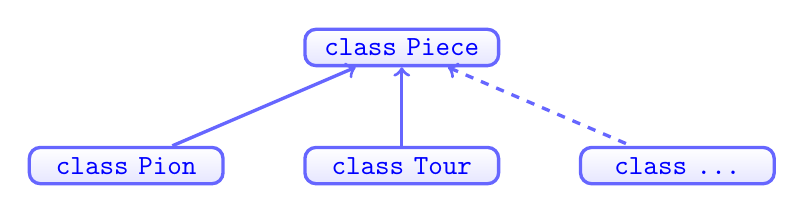
\begin{tikzpicture}[
      grow=down,
      linet/.style={very thick,draw=blue!60,
        shorten >=0pt, shorten <=0pt, <-},
      punkt/.style={rectangle, rounded corners, shade, top color=white,
        bottom color=blue!10, draw=blue!60, very
        thick, text centered, text width=6em}
    ]
    \ttfamily\color{blue}
    \path (0,0) node(a) [punkt] {class Piece}
    (-3.5,-1.5) node(b) [punkt] {class Pion}
    (+0.0,-1.5) node(c) [punkt] {class Tour}
    (+3.5,-1.5) node(d) [punkt] {class ...};
    \draw[linet] (a) -- (b);
    \draw[linet] (a) -- (c);
    \draw[linet, dashed] (a) -- (d);
  \end{tikzpicture}
\end{center}

\begin{itemize}
\item La classe \texttt{Piece} est par nature \structure{une classe abstraite} : elle déclare
des méthodes virtuelles pures : \texttt{affiche()}, \texttt{deplacement()}

\item La définition n'intervient que dans les classes dérivées qui spécialisent les
méthodes en fonction de leur besoin
\end{itemize}
\end{frame}


%---------------------------------------------------------------------------------

\begin{frame}[fragile]{Classes abstraites}
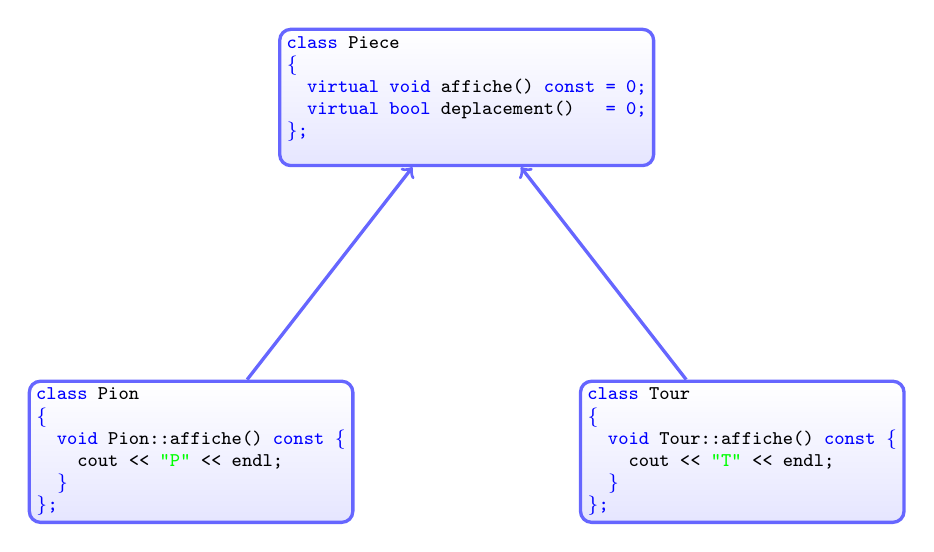
\begin{tikzpicture}[
    grow=down,
    linet/.style={very thick,draw=blue!60,
      shorten >=0pt, shorten <=0pt, <-},
    punkt/.style={rectangle, rounded corners, shade, top color=white,
      bottom color=blue!10, draw=blue!60, very
      thick, text centered, align=left}
  ]
  \ttfamily\scriptsize\color{blue}
  \path (0,0) node(a) [punkt] {
    class \ttb{Piece}\\
    \{\\
    ~~virtual void \ttb{affiche()} const = 0;\\
    ~~virtual bool \ttb{deplacement()}~~~= 0;\\
    \};\\
  }
  
  (-3.5,-4.5) node(b) [punkt] {
    class \ttb{Pion}\\
    \{\\
    ~~void \ttb{Pion::affiche()} const \{\\
    ~~~~\ttb{cout <<} \ttg{"P"} \ttb{<< endl;}\\
    ~~\}\\
    \};
  }
  (+3.5,-4.5) node(c) [punkt] {
    class \ttb{Tour}\\
    \{\\
    ~~void \ttb{Tour::affiche()} const \{\\
    ~~~~\ttb{cout <<} \ttg{"T"} \ttb{<< endl;}\\
    ~~\}\\
    \};
  };
  \draw[linet] (a) -- (b);
  \draw[linet] (a) -- (c);
\end{tikzpicture}

\end{frame}

%-------------------------------------------------------------

\begin{frame}[fragile]{On résume tout}
\begin{minted}[fontsize=\footnotesize,samepage,mathescape,xrightmargin=0.5cm,xleftmargin=0.5cm]{c++}
#include "Pion.h"
#include "Tour.h"

int main()
{
  std::vector< Piece* > pieces;  // conteneur d'objets hétérogènes

  // instanciation d'objets non-abstraits
  pieces.push_back( new Pion );
  pieces.push_back( new Tour );

  for (size_t i = 0; i < pieces.size(); ++i)
    pieces[i]->affiche();  // polymorphisme à l'œuvre
}
\end{minted}

\pause
\begin{center}
Étant donné le canevas / l'\structure{interface} fournie par la déclaration de la classe \texttt{Piece}, libre à chaque classe fille d'implémenter, de façon indépendante, ces fonctionnalités.
\end{center}
\end{frame}

%-------------------------------------------------------------

\begin{frame}{Utilisations de l'héritage}
\begin{itemize}

\item Extension (ajout de fonctionnalités...) d'une classe existante, même tierce.

\item Structuration : Découpage d'un programme en sous-programmes, en composants non-indépendants $\to$~découplage de concepts distincts, évolutivité, modularité $\to$ TD 4

\item Sous-typage et création d'une famille d'objets (relation de type \structure{\textbf{est un}}). Utile pour des systèmes de simulation, pour la représentations d'objets physiques ou logiciels (interfaces utilisateurs...). Polymorphisme. $\to$ TD 5

\item Spécifications d'interfaces, d'APIs (classes virtuelles pures)

\end{itemize}
\end{frame}

%-------------------------------------------------------------

\begin{frame}[fragile]{Et dans d'autres langages ?}
L'héritage diffère notablement entre les langages orientés objets.\\

En Python :
\begin{minted}[fontsize=\footnotesize,xrightmargin=0.5cm,xleftmargin=0.5cm]{python}
class Polygone:

  def affiche(self):
    # ...

class Rectange (Polygone):

  def __init__(self):
    super.__init__()

  def affiche(self):
    Polygon.affiche()
    # ...
\end{minted}
\end{frame}

\end{document}
